\section{Results}
\label{sec:results}

\subsection{Effect of the Split Protocol}
\label{sec:leak}
Table~\ref{tab:leak} evaluates the same 21 raw columns under three protocols with an untuned gradient-boosting classifier, quantifying a known pitfall~\cite{kapoor2023leakage,kaufman2012leakage} on these data. Oversampling every discomfort grade to 5,243 samples before a 70/15/15 row split, the protocol of the earlier version of this study, gives \LeakOldAcc\,\% accuracy and ROC-AUC \LeakOldRocAuc; \LeakDupPct\,\% of the positive test rows have an exact duplicate in training. A row-level split without oversampling still gives ROC-AUC \LeakRowRocAuc, whereas a session-grouped split gives \LeakGrpRocAuc{} (MCC \LeakGrpMCC). The earlier E-DDQN implementation behaves alike (MCC \OrigOldMCC{} vs.\ \OrigGrpMCC). Near-perfect scores on these data thus measure recognition of seen sessions, without any RL; all further results use the grouped protocol of Fig.~\ref{fig:protocol}.

\begin{table*}[t]
\centering
\caption{Effect of the evaluation protocol on the same data (21 raw columns; test-split metrics). ``Proxy'': reconstruction of the earlier protocol, whose 41-feature input files were not available.}
\label{tab:leak}
\resizebox{\textwidth}{!}{\begin{tabular}{llccccc}
\toprule
Model & Evaluation protocol & Acc. & Recall & Spec. & MCC & ROC-AUC \\
\midrule
HGB & Oversample to 5,243/grade, then 70/15/15 row split (earlier protocol) & 97.6 & 99.8 & 91.0 & 0.935 & 0.995 \\
HGB & Row-level random split, no oversampling & 95.3 & 94.1 & 96.3 & 0.905 & 0.992 \\
HGB & Grouped 5-fold split (session-linkage groups) & 52.2 & 33.6 & 66.9 & 0.005 & 0.523 \\
E-DDQN (earlier code) & Earlier script, earlier protocol (proxy) & 95.2 & 99.2 & 83.1 & 0.870 & -- \\
E-DDQN (earlier code) & Earlier script, grouped split (proxy) & 41.1 & 92.1 & 7.7 & $-$0.004 & -- \\
\bottomrule
\end{tabular}
}
\end{table*}

\subsection{Session-Grouped Comparison under the 5:1 Cost (RQ2)}
\label{sec:main}
Table~\ref{tab:main} gives every model's result, with thresholds chosen on validation groups only. Two facts dominate. First, discrimination is weak once sessions and groups are not shared: the best primary ROC-AUC is \HGBCostRocAucMean{} (HGB) and \RFCostRocAucMean{} (RF), and the best PR-AUC \DQNCostPrAucMean{} (DQN) against a prevalence of 0.44. Second, under a 5:1 cost every cost-optimal operating point lies near ``always alarm'' (cost \AlwaysCost): recall is high, but \DOneFPRMin--\DOneFPRMax\,\% of non-event seconds trigger an alarm. The random forest has the lowest cost (seed mean \RFCostCostMean$\pm$\RFCostCostSD; ensemble \PHEnsRFCost; point estimates, differences among supervised models not tested).

With its primary search draw, E-DDQN has the highest cost and lowest ROC-AUC of the \nModels{} primary models: cost \EDDQNCostCostMean$\pm$\EDDQNCostCostSD{} (ensemble \PHEnsEDDQNCost), recall \EDDQNCostRecallMean\,\%, specificity \EDDQNCostSpecMean\,\%, ROC-AUC \EDDQNCostRocAucMean{} (ensemble \EDDQNCostRocAucEns, 95\,\% CI \EDDQNCIRocAucLo{} to \EDDQNCIRocAucHi, which includes chance). Its seed-ensemble cost exceeds the random forest's in \PHFoldsEDDQNWorseRF{} of 5 outer folds, by \PHFoldDiffEDDQNRFMin{} to \PHFoldDiffEDDQNRFMax. The standard DQN reaches cost \DQNCostCostMean{} and ROC-AUC \DQNCostRocAucMean, E-CB \ECBCostCostMean{} and \ECBCostRocAucMean.

\begin{table*}[t]
\centering
\caption{Session-grouped comparison (rule D1; \nSamplesEval{} outer-test samples; recall, specificity, balanced accuracy in \%). Left: mean~$\pm$~SD over five seeds. Right: seed ensemble, used for all paired tests and confidence intervals; FN and FP are exact counts. Bold: proposed model and lowest primary cost. HGB, logistic regression and the post-hoc baselines are deterministic (SD = 0). Further metrics: Supplementary Sec.~S3.1.}
\label{tab:main}
\resizebox{\textwidth}{!}{\begin{tabular}{lccccccc|ccccc}
\toprule
 & \multicolumn{7}{c|}{Mean $\pm$ SD over five seeds} & \multicolumn{5}{c}{Seed ensemble (paired tests)} \\
Model & Recall & Spec. & Bal.\ acc. & MCC & Cost$_{5:1}$ & ROC-AUC & PR-AUC & Recall & Spec. & Cost$_{5:1}$ & FN & FP \\
\midrule
\textbf{E-DDQN} & 93.4$\pm$2.5 & 7.4$\pm$2.7 & 50.4$\pm$1.2 & 0.016$\pm$0.054 & 0.663$\pm$0.048 & 0.538$\pm$0.016 & 0.483$\pm$0.019 & 90.4 & 8.1 & 0.726 & 400 & 4,820 \\
E-CB & 97.1$\pm$2.9 & 8.4$\pm$2.8 & 52.8$\pm$1.2 & 0.122$\pm$0.052 & 0.575$\pm$0.055 & 0.653$\pm$0.011 & 0.562$\pm$0.006 & 96.6 & 14.6 & 0.552 & 140 & 4,480 \\
DQN & 95.2$\pm$2.7 & 14.5$\pm$4.9 & 54.8$\pm$1.6 & 0.158$\pm$0.038 & 0.584$\pm$0.040 & 0.661$\pm$0.013 & 0.595$\pm$0.022 & 96.9 & 16.3 & 0.536 & 129 & 4,391 \\
CS-MLP & 99.4$\pm$0.7 & 2.8$\pm$1.9 & 51.1$\pm$0.8 & 0.072$\pm$0.049 & 0.557$\pm$0.012 & 0.644$\pm$0.018 & 0.521$\pm$0.022 & 99.4 & 6.1 & 0.537 & 23 & 4,925 \\
LogReg & 99.1$\pm$0.0 & 8.1$\pm$0.0 & 53.6$\pm$0.0 & 0.167$\pm$0.000 & 0.532$\pm$0.000 & 0.626$\pm$0.000 & 0.576$\pm$0.000 & 99.1 & 8.1 & 0.532 & 36 & 4,817 \\
HGB & 97.0$\pm$0.0 & 14.6$\pm$0.0 & 55.8$\pm$0.0 & 0.197$\pm$0.000 & 0.543$\pm$0.000 & 0.692$\pm$0.000 & 0.593$\pm$0.000 & 97.0 & 14.6 & 0.543 & 124 & 4,479 \\
RF & 98.5$\pm$0.3 & 18.2$\pm$0.7 & 58.3$\pm$0.3 & 0.266$\pm$0.004 & \textbf{0.491$\pm$0.003} & 0.688$\pm$0.002 & 0.548$\pm$0.001 & 98.7 & 18.3 & \textbf{0.485} & 54 & 4,281 \\
\midrule
\multicolumn{13}{l}{\emph{Post-hoc exposure-time baselines (added after the primary analysis)}} \\
Time-LR (elapsed time) & 96.7$\pm$0.0 & 15.0$\pm$0.0 & 55.8$\pm$0.0 & 0.194$\pm$0.000 & 0.548$\pm$0.000 & 0.704$\pm$0.000 & 0.605$\pm$0.000 & 96.7 & 15.0 & 0.548 & 138 & 4,457 \\
Time+game HGB & 97.4$\pm$0.0 & 17.6$\pm$0.0 & 57.5$\pm$0.0 & 0.239$\pm$0.000 & 0.517$\pm$0.000 & 0.676$\pm$0.000 & 0.550$\pm$0.000 & 97.4 & 17.6 & 0.517 & 107 & 4,319 \\
\midrule
Always alarm & 100.0 & 0.0 & 50.0 & 0.000 & 0.558 & -- & -- & 100.0 & 0.0 & 0.558 & 0 & 5,243 \\
Never alarm & 0.0 & 100.0 & 50.0 & 0.000 & 2.208 & -- & -- & 0.0 & 100.0 & 2.208 & 4,147 & 0 \\
\bottomrule
\end{tabular}
}
\end{table*}

\emph{Exposure-time baselines (post hoc).} Time-LR, a logistic regression on elapsed time alone, reaches ROC-AUC \PHTimeLRRocAucMean{} (Fig.~\ref{fig:roc}); within folds the random forest is slightly higher (\PHWfRFAuc{} vs.\ \PHWfTimeLRAuc) and E-DDQN lowest (\PHWfEDDQNAuc). Time-LR's ROC-AUC does not differ significantly from the random forest's (difference \PHTimeLRvsRFAuc, CI \PHTimeLRvsRFAucLow{} to \PHTimeLRvsRFAucHigh), and the wide interval does not establish equivalence either. At the 5:1 operating point the random forest has a lower cost than Time-LR (\PHEnsRFCost{} vs.\ \PHEnsTimeLRCost; group bootstrap $p=$\,\PHTimeLRvsRFCostP, sign-flip $p=$\,\PHSfTimeLRvsRFP; approximate), so the evidence that its additional inputs help is suggestive, not conclusive. Time-LR ranks seconds better than the primary E-DDQN (ROC-AUC difference \PHTimeLRvsEDDQNAuc, CI \PHTimeLRvsEDDQNAucLow{} to \PHTimeLRvsEDDQNAucHigh). No primary model was shown to discriminate better than a population onset curve, as long documented for exposure duration~\cite{kennedy2000duration}; modest gains remain possible within the wide intervals.

\begin{figure}[t]
\centering
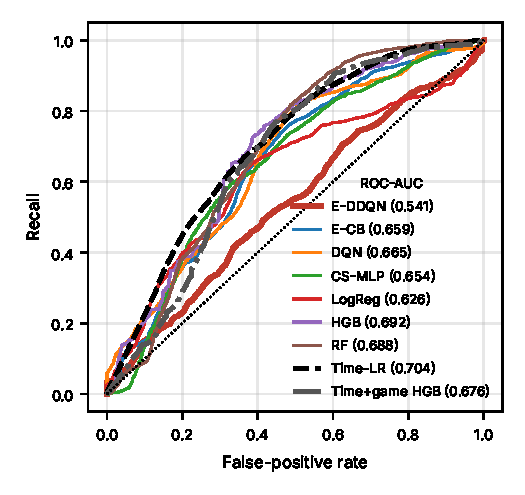
\includegraphics[width=\columnwidth]{figs/posthoc_roc.pdf}
\caption{ROC curves of the seed-ensemble scores, pooled over the outer-test folds, for the primary models and the exposure-time baselines (dashed). Legend: ensemble ROC-AUC.}
\label{fig:roc}
\end{figure}

\subsection{Statistical Comparison}
\label{sec:stats}
Table~\ref{tab:paired} compares E-DDQN with each primary model on identical test samples (seed ensembles). E-DDQN's ensemble cost exceeds the others' by \PairDOneECBCostDiff{} to \PairDOneRFCostDiff; these differences are larger than those of seed means (\PHMeanDiffDQN{} to \PHMeanDiffRF) because E-DDQN's ensemble is worse than its average seed. After Holm adjustment, only the difference from the random forest is significant under the primary group bootstrap (\PairDOneRFCostDiff, 95\,\% CI \PairDOneRFCostLo{} to \PairDOneRFCostHi; $p=$\,\PHHolmRF); the other five adjusted $p$-values lie between \PHHolmECB{} and \PHHolmHGB, and the difference from the standard DQN (\PairDOneDQNCostDiff) is not significant (unadjusted $p=$\,\PairDOneDQNPboot). The sign-flip sensitivity analysis gives $p=$\,\PHSfRFHolm{} (Holm) for the random-forest comparison. The direction is stable---the session-level bootstrap gives the same pattern (Holm $p=$\,\PHSesRFHolm) and no leave-one-group-out deletion changes the sign (\PHJkEDDQNvsRFMin{} to \PHJkEDDQNvsRFMax)---but because the difference is significant under the primary procedure only, it is not firmly established, and we do not conclude that the random forest is superior.

Against always alarming, no model's cost difference is significant after Holm adjustment with linkage groups as units (random forest \PHAlwRFGrp, CI \PHAlwRFGrpLow{} to \PHAlwRFGrpHigh, adjusted $p=$\,\PHAlwRFGrpHolm; E-DDQN \PHAlwEDDQNGrp, adjusted $p=$\,\PHAlwEDDQNGrpHolm). This reflects the strength of the evidence, not demonstrated equivalence; resampling sessions instead, which ignores dependence between linked sessions, leaves the random forest's advantage significant (adjusted $p=$\,\PHAlwRFSesHolm, approximate).

\begin{table*}[t]
\centering
\caption{Paired comparisons with E-DDQN (A) on the same \nSamplesEval{} test samples (seed ensembles, rule D1). $b$: A correct, B wrong; $c$: A wrong, B correct. $\Delta$Cost: difference of seed-ensemble costs; CI and $p_{\text{group}}$ from 2,000 group-bootstrap replicates (unadjusted; Holm-adjusted values in the text); $p_{\text{exact}}$: sample-level McNemar test, which ignores within-session dependence.}
\label{tab:paired}
\footnotesize
\begin{tabular}{lcccccccc}
\toprule
B (vs. A = E-DDQN) & $b$ & $c$ & err$_A$ & err$_B$ & $\chi^2_{cc}$ & $p_{\text{exact}}$ & $\Delta$Cost$_{5:1}$ (A$-$B) [95\% CI] & $p_{\text{group}}$ \\
\midrule
E-CB & 299 & 899 & 5,220 & 4,620 & 299.5 & $<$0.001 & +0.175 [+0.016, +0.448] & 0.014 \\
DQN & 297 & 997 & 5,220 & 4,520 & 377.6 & $<$0.001 & +0.190 [$-$0.017, +0.493] & 0.079 \\
CS-MLP & 402 & 674 & 5,220 & 4,948 & 68.3 & $<$0.001 & +0.190 [+0.005, +0.485] & 0.039 \\
LogReg & 389 & 756 & 5,220 & 4,853 & 117.0 & $<$0.001 & +0.194 [+0.011, +0.477] & 0.026 \\
HGB & 203 & 820 & 5,220 & 4,603 & 370.9 & $<$0.001 & +0.183 [+0.011, +0.460] & 0.035 \\
RF & 293 & 1,178 & 5,220 & 4,335 & 531.2 & $<$0.001 & +0.242 [+0.052, +0.528] & 0.001 \\
\bottomrule
\end{tabular}

\end{table*}

\subsection{Operating Points and Cost Ratios}
\label{sec:op}
With the untuned rule D0 (for E-DDQN the greedy policy, an effective cut-off of \SSEDDQNCutMin--\SSEDDQNCutMax{} on $P(y=1\mid s)$) E-DDQN reaches recall \EDDQNBayesRecallMean\,\% at specificity \EDDQNBayesSpecMean\,\% (cost \EDDQNBayesCostMean), the random forest \RFBayesRecallMean\,\% at \RFBayesSpecMean\,\% (\RFBayesCostMean); under a validation recall of at least 0.95 the random forest again has the lowest cost (\RFRecCostMean; E-DDQN \EDDQNRecCostMean; Supplementary Sec.~S9.3). At validation-matched recall targets, E-DDQN's thresholds transfer worst (Supplementary Sec.~S9.4). Since the reward encodes the same operating point as a cost-weighted classifier (Eq.~\eqref{eq:margin}), it provided no advantage that cost weighting plus a validation-chosen threshold did not.

The cost curves (Fig.~\ref{fig:costcurves}) show that this negative result does not depend on the 5:1 ratio. At $R=1.5$--2, the relative costs of all models except E-DDQN lie between \PHCcLowRMin{} and \PHCcLowRMax; as $R$ grows, always alarming becomes nearly optimal and models that still miss events rise above 1 (at $R=20$: E-DDQN \PHCcEDDQNTwenty, DQN \PHCcDQNTwenty). The lowest relative cost over all models and ratios is \PHCcMinAll{} (random forest, $R=\PHCcMinAllRatio$), so no model removes more than about \PHCcMinAllReduction\,\% of the cost of the better trivial policy at any ratio (point estimates).

\begin{figure}[t]
\centering
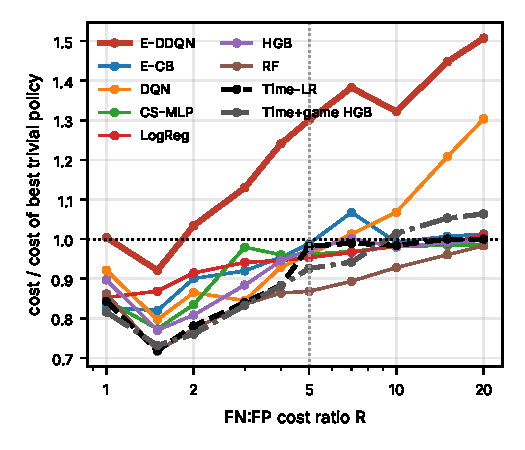
\includegraphics[width=\columnwidth]{figs/posthoc_cost_curves.pdf}
\caption{Validation-chosen cost curves (post hoc): for each cost ratio $R$, the threshold minimizing $R\,\mathrm{FN}+\mathrm{FP}$ on validation predictions is applied to the test fold; the seed-ensemble test cost is divided by that of the better trivial policy. Values below 1 beat both trivial policies; dotted line: $R=5$.}
\label{fig:costcurves}
\end{figure}

\emph{Event level.} At the cost-optimal operating points every model flags almost every session: E-DDQN alarms on \EDDQNEvFreeAlarm\,\% of the seconds of the \nEventFreeSessions{} event-free sessions and \EDDQNEvPreAlarm\,\% of pre-onset seconds (random forest \RFEvFreeAlarm\,\% and \RFEvPreAlarm\,\%), so events are ``detected'' with zero median delay by construction, not by discrimination.

\subsection{Why E-DDQN Under-Performs in the Primary Analysis}
\label{sec:why}
Validation selected $\gamma=$ \EDDQNGammas{} for E-DDQN's five folds and the questionnaire indicators in \EDDQNnProfile{} of 5 folds.

\emph{Search draw (pre-specified experiment).} With two further random draws, E-DDQN never had a significantly lower cost than the standard DQN (ensemble differences \SDCostDiffMin{} to \SDCostDiffMax; smallest $p=$\,\SDCostPMin; rule R1). Its own result depended strongly on the draw (rule R2): seed-mean cost \SDEDDQNCostMin--\SDEDDQNCostMax{} and within-fold ROC-AUC \SDEDDQNWfMin, the lowest of the primary models, to \SDEDDQNWfMax, close to the highest (RF \PHWfRFAuc); the DQN varied less (\SDDQNWfMin--\SDDQNWfMax). The ranking of the two agents reversed: the DQN ranked seconds better with draw~1 ($p=$\,\SDPairOneAucP, approximate), E-DDQN with draw~2 ($p=$\,\SDPairTwoAucP). The primary draw offered only \PHDrawExposureEDDQN{} exposure-only E-DDQN configurations (DQN \PHDrawExposureDQN), and the selection criterion, nearly flat near always alarming (\PHSelCostMin--\PHSelCostMax{} vs.\ \AlwaysCost), let questionnaire-based configurations win on validation and then lose most on test (selection optimism \EDDQNOptGap{} vs.\ \RFOptGap--\ECBOptGap{} for the other models; Supplementary Sec.~S9.5)~\cite{varma2006bias}. Restricted to exposure features, E-DDQN's within-fold ROC-AUC (\SDEDDQNExposureWfAuc) was within \SDExposureGap{} of the DQN's (rule R3).

\emph{Questionnaire indicators (exploratory).} Across the seven primary models, the \PHFsProfile{} selected configurations with questionnaire indicators rank worse within folds than the \PHFsNoProfile{} without them (deviation from the fold mean \PHFsDevProfile{} vs.\ \PHFsDevNoProfile; Supplementary Sec.~S5.9). With \nGroupsEval{} groups such indicators may fit group-level label rates that do not transfer; feature sets were selected, not assigned, so this suggests but does not establish a cause.

\emph{Bootstrapping.} With E-DDQN's configurations fixed, $\gamma=0$ raises ROC-AUC only from \EDDQNCostRocAucMean{} to \AblGammaZeroCostRocAuc{} (Table~\ref{tab:ablation}), and in draw~2 E-DDQN reached its best ranking with $\gamma=0.99$ in \SDEDDQNDrawTwoStrongGammaFolds{} of 5 folds. Q-values stay finite but exceed the return bound $r_{\max}/(1-\gamma)$ by up to a factor of \PHQRatioMaxEDDQN{} (Supplementary Sec.~S5.6).

Together these results suggest that sensitivity to the search draw, combined with noisy validation-based selection, contributes substantially to E-DDQN's weak primary result. They do not isolate a single cause---draw, feature sets, discount factors and other hyper-parameters varied together---and they do not show that any E-DDQN component helps a configuration that ranks well.

\subsection{Component Ablation and Reward Ratio}
\label{sec:ablation}
Table~\ref{tab:ablation} removes or changes one component of E-DDQN at a time while keeping the configuration selected for each outer fold fixed (five seeds; same protocol). No formal test was performed, so the differences below are point estimates. Because the selected configurations already used no warm-up in four of the five folds, the ``no warm-up'' variant differs from the full model only in the remaining fold. This analysis and the reward-ratio analysis below hold E-DDQN's primary (draw-1) configurations fixed, which rank weakly (Section~\ref{sec:why}); they cannot show whether a component helps a configuration that ranks well. Every variant ranks seconds only weakly (ROC-AUC \AblSoftCostRocAuc--\AblGammaZeroCostRocAuc, where 0.5 is chance). No single change moves the cost by more than about one seed standard deviation of the full model (\EDDQNCostCostMean$\pm$\EDDQNCostCostSD). The lowest cost is obtained by \emph{replacing} the asymmetric reward with the symmetric $\pm1$ reward (\AblAsymCostCost) and the highest ROC-AUC by switching off bootstrapping ($\gamma=0$; \AblGammaZeroCostRocAuc); hard target copies (\AblSoftCostCost), no dueling head (\AblDuelCostCost), uniform replay (\AblBalCostCost), no warm-up (\AblWarmCostCost) and toggling full-information replay (\AblFullCostCost) leave the cost essentially unchanged, and removing the double estimator slightly increases it (\AblDoubleCostCost). None of these components can be credited with a gain in safety or accuracy. Every variant is scored on the same nominal implied-probability scale and thresholded with the same rules, so the reward table can act only through the learned scores; at the fixed cut-off $\hat p\ge1/6$ (rule D0) the symmetric-reward variant is not worse either (cost \AblAsymBayesCost{} vs.\ \EDDQNBayesCostMean), although the effective position of that cut-off on $P(y=1\mid s)$ differs between the variants (Section~\ref{sec:formulation}).

\begin{table*}[t]
\centering
\caption{Leave-one-component-out ablation of E-DDQN (selected configuration per outer fold held fixed; rule D1; mean over 5 seeds, cost $\pm$ SD). The no-warm-up variant changes only the one fold whose selected configuration used warm-up.}
\label{tab:ablation}
\footnotesize
\begin{tabular}{lccccc}
\toprule
Variant & Recall & Spec. & Cost$_{5:1}$ & ROC-AUC & PR-AUC \\
\midrule
Full E-DDQN (selected) & 93.4 & 7.4 & 0.663$\pm$0.048 & 0.538 & 0.483 \\
\midrule
full-information replay toggled & 93.7 & 5.4 & 0.667$\pm$0.106 & 0.563 & 0.500 \\
symmetric $\pm$1 reward instead of asymmetric & 94.8 & 8.6 & 0.625$\pm$0.038 & 0.572 & 0.517 \\
uniform instead of class-balanced replay & 94.3 & 4.3 & 0.660$\pm$0.045 & 0.554 & 0.486 \\
no double estimator (max-operator target) & 93.1 & 5.3 & 0.681$\pm$0.086 & 0.543 & 0.491 \\
no dueling head & 94.6 & 5.8 & 0.644$\pm$0.059 & 0.559 & 0.494 \\
hard target copy every 10 updates & 94.9 & 6.5 & 0.634$\pm$0.043 & 0.529 & 0.472 \\
no warm-up & 93.8 & 7.1 & 0.656$\pm$0.049 & 0.547 & 0.497 \\
$\gamma=0$ (contextual bandit) & 94.4 & 6.4 & 0.645$\pm$0.070 & 0.576 & 0.510 \\
\bottomrule
\end{tabular}

\end{table*}


Varying the reward's regret ratio from 1:1 to 10:1 with E-DDQN's configurations fixed moves the greedy policy along the trade-off as Eq.~\eqref{eq:margin} predicts (recall \RatioArgOneRecall\,\% at 1:1, \RatioArgFiveRecall\,\% at 5:1, \RatioArgOneZeroRecall\,\% at 10:1), but once the threshold is chosen on validation data all ratios end at similar costs (\RatioTunedOneCost--\RatioTunedOneZeroCost; within one seed SD, untested; Supplementary Sec.~S9.6): the ratio sets the default operating point, not the discrimination.

\subsection{Telemetry-Perturbation Stress Test (RQ3)}
\label{sec:attack}
Under the whole-session perturbations, \AttAucFracSmall\,\% of the model--scenario ROC-AUC values change by less than 0.03 and none by more than \AttAucMaxAbsChange{} (Supplementary Sec.~S9.7). This feature-space stress test gives no evidence of robustness: \PHFsExposure{} of \PHFsTotal{} selected configurations use exposure features, which the perturbations barely touch, and a shift applied to every session alike need not reorder scores. At fixed thresholds the adaptive adversary lowers recall on event seconds by \AttEvasionDropMin--\AttEvasionDropMax{} percentage points and raises false-positive rates to \EDDQNAttWorstFPR--100\,\% (Supplementary Sec.~S4.3). SHAP attributions of E-DDQN's $\Delta Q$ are dominated by \ShapTopFive{} (Supplementary Sec.~S9.8): exposure and questionnaire inputs rather than instantaneous telemetry, consistent with the exposure-time baselines; since the primary E-DDQN ranks near chance, they describe what it uses, not a validated signal.
